\section{Results}
\label{sec:results}

The results are reported per research question. Unless stated otherwise, a score is the mean
within-compound Spearman correlation of Equation~\ref{eq:metric}, out of fold over held-out cell lines,
averaged over the \NPanel{} panel compounds and three seeds \cite{spearman1904,dreval}.
% ; each value is
% read from a committed artifact under \code{notebooks/outputs/}, named in \code{results\_numbers.tex}.

\subsection{Prediction from single cells with bulk labels}
\label{sec:results-q1}

Table~\ref{tab:sweep} reports the score of every configuration, to establish whether any configuration
predicts response and how the per-cell model compares with the ridge control; the focus is the PCA
column, which holds both the highest score and the control. Rows are the six combinations of loss and
density exponent $\alpha$ for the MLP, followed by the ridge regression on cell-line means; columns are
the two representations, and the highest score is set in bold \cite{hoerl1970,dir}. All six PCA
configurations scored between \SpSweepLo{} and \SpBest{}, the highest score being reached with MAE and
$\alpha = 0.5$, and the ridge regression scored \RidgePca{}. Under the decision rule no configuration
displaced the incumbent, unweighted MAE at \SwPcaMaeZero{}: the \SpBest{} configuration was better on order
but worse on values and spread by more than their seed bands.
% (\code{panel\_metrics.csv})
One configuration (PCA, MSE, $\alpha = 0$) differed between two identical
executions, \SwPcaMseZeroAlt{} against \SpSweepLo{}; the other thirteen entries agreed to four decimals.
% (\code{panel\_execution\_band.csv})

\begin{table}[h]
\caption{\textbf{Out-of-fold scores of all configurations.} Mean within-compound Spearman correlation
between predicted and true AUC across held-out cell lines (Equation~\ref{eq:metric}), for the MLP under
each loss (MSE, MAE) and density exponent $\alpha$ (Equation~\ref{eq:density}; $\alpha = 0$ is
unweighted), and for the ridge regression on cell-line means, on either representation. Five-fold CV
grouped by cell line over \NLinesCV{} lines, \NPanel{} compounds, mean over seeds 42--44; higher is
better, 0 is no ranking skill. Bold: highest score.
% Read from \code{panel\_per\_drug\_correlation.csv}
% and \code{panel\_ridge\_baseline.csv} (\code{notebooks/4a\_percell\_training.ipynb}).
}
\label{tab:sweep}
\centering
\begin{tabular}{llcc}
\toprule
Model & Loss, $\alpha$ & PCA & scGPT \\
\midrule
MLP & MSE, 0   & \SwPcaMseZero & \SwScgptMseZero \\
MLP & MSE, 0.5 & \SwPcaMseHalf & \SwScgptMseHalf \\
MLP & MSE, 1   & \SwPcaMseOne  & \SwScgptMseOne \\
MLP & MAE, 0   & \SwPcaMaeZero & \SwScgptMaeZero \\
MLP & MAE, 0.5 & \textbf{\SwPcaMaeHalf} & \SwScgptMaeHalf \\
MLP & MAE, 1   & \SwPcaMaeOne  & \SwScgptMaeOne \\
\midrule
Ridge (line means) & --- & \RidgePca & \RidgeScgpt \\
\bottomrule
\end{tabular}
\end{table}

Figure~\ref{fig:labelquality} breaks the highest-scoring configuration down by compound, to test
whether the variation between compounds follows the quality of their labels; the focus is the relation
between the two axes rather than any single compound. Each point is one
compound, placed by the share of its dose--response curves that are flat (logarithmic axis) and by its
score; the compounds at the extremes and the exception are labelled in bold. Scores ranged from
\SpDrugLo{} for cisplatin to \SpDrugHi{} for dasatinib, and the share of flat curves from $0$ to
\PlatinFracNs\,\%. The two were correlated, Spearman $\rho = \FlatRho$ ($p = \FlatP$, $n = 11$):
compounds with more flat curves scored lower, cisplatin having both the largest share and the lowest
score, while crizotinib had no flat curves and a middling score. Across all \NCurves{} curves behind the
panel, the median $R^2$ of the fits was \CurveMedRsq{}, \CurveFracLowRsq\,\% had $R^2 < 0.5$, and
\CurveFracNs\,\% were flat; cisplatin's median $R^2$ was \PlatinMedRsq{}.

\begin{figure}[t]
\centering
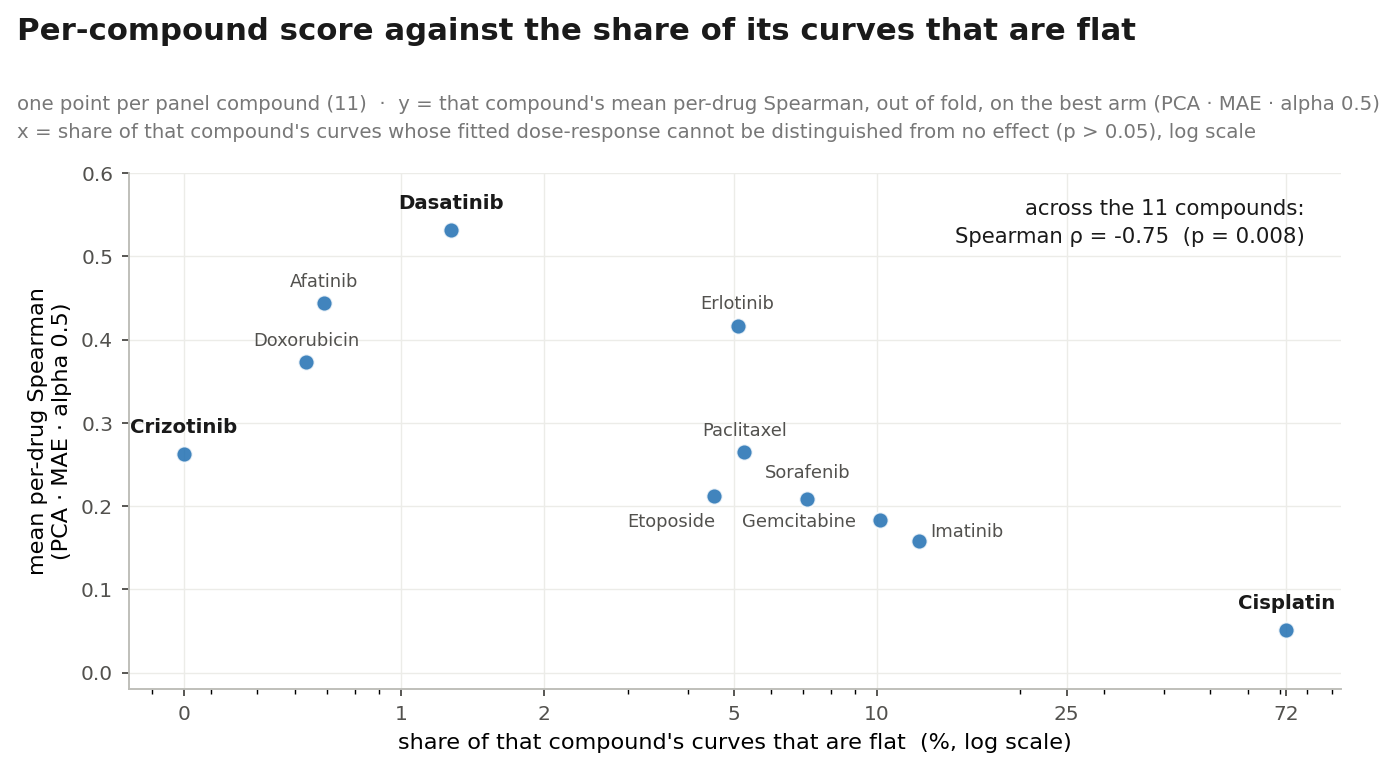
\includegraphics[width=0.85\textwidth]{label_quality.png}
\caption{\textbf{Per-compound score against label quality.} One point per panel compound
($n = \NPanel$). Vertical axis: mean within-compound Spearman correlation, out of fold, of the
highest-scoring configuration (PCA, MAE, $\alpha = 0.5$). Horizontal axis: share of the compound's CurveCurator fits that are flat, i.e.\ cannot reject a
no-effect null ($p > 0.05$), on a logarithmic scale. Bold labels mark the highest (dasatinib) and
lowest (cisplatin) scores and the exception to the trend (crizotinib). The inset reports the Spearman
correlation over the eleven compounds.
% Generated by \code{docs/make\_figures.py} from
% \code{diagnostics/label\_quality\_vs\_performance.csv} and \code{panel\_per\_drug\_correlation.csv}.
}
\label{fig:labelquality}
\end{figure}

The share of the score that reflects general cell-line fragility rather than compound-specific
response was measured next, because LCO cannot remove it \cite{dreval}. Averaged over the six
configurations, the predictions correlated with fragility at \FragRhoPca{} in the PCA arm and
\FragRhoScgpt{} in the scGPT arm, and controlling for it by Equation~\ref{eq:partial} lowered the score
from \FragRawPca{} to \FragPartialPca{} ($-\FragCostPca\,\%$) and from \FragRawScgpt{} to
\FragPartialScgpt{} ($-\FragCostScgpt\,\%$).
% (\code{bias\_accounting.csv})
Figure~\ref{fig:lpo} shows how much a line's identity alone predicts when the protocol allows it to;
the focus is the size of that baseline relative to the scores above. The two bars are DrEval's LPO
baselines that use no expression: the mean response of the line (black) reached a mean within-compound
correlation of \LpoLineMean{}, and the mean response of its lineage (grey) \LpoTissueMean{}.
% (\code{dreval\_lpo\_results.csv})

\begin{figure}[t]
\centering
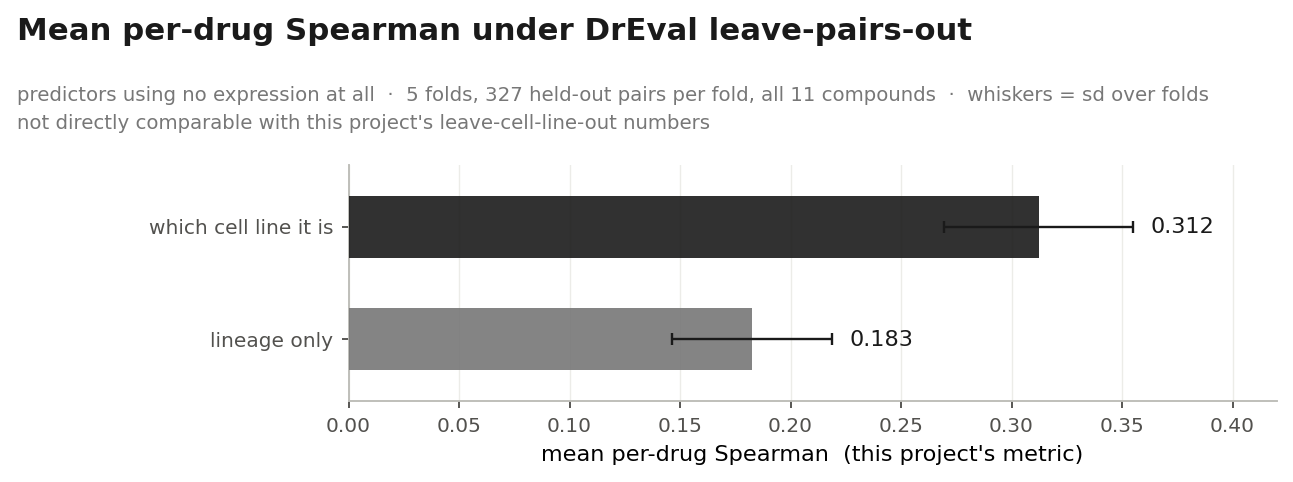
\includegraphics[width=0.8\textwidth]{lpo_bias.png}
\caption{\textbf{What cell-line identity alone predicts.} Mean within-compound Spearman correlation of
two DrEval baselines under leave-pairs-out (LPO) evaluation, in which held-out (line, compound) pairs
belong to lines seen in training: predicting each line's mean response (black, ``which cell line it
is'') and each lineage's mean response (grey, ``lineage only''). Neither uses expression. Five folds of
about 383 held-out pairs over the \NPanel{} compounds; whiskers are the SD over folds. LPO scores are not
comparable with the LCO scores of Table~\ref{tab:sweep}.
% Generated by \code{docs/make\_figures.py} from
% \code{dreval\_lpo\_results.csv} (\code{scripts/evaluation/dreval\_lpo.py}).
}
\label{fig:lpo}
\end{figure}

Finally, the per-cell model was set against the two line-level controls and the unselected catalogue
\cite{hoerl1970,breiman2001}. The ridge regression on cell-line means scored \RidgePca{} against
\SpBest{}. On DrEval's LCO benchmark the per-compound random forest scored \DrRfNorm{} on the normalised
metric against \DrMlpNorm{} for the MLP, with a fold SD of \DrRfSd{} against \DrMlpSd{}, and both exceeded
DrEval's naive baselines, which score zero on that metric \cite{dreval}. Over all \NDrugsModelled{}
compounds the score was \SpAllDrugs{}, at most \NullGainMax{} above a per-compound constant.
% (\code{panel\_heads\_summary.csv})

\subsection{scGPT against PCA}
\label{sec:results-q2}

The two arms were compared first on the trained models and then on their inputs.
The PCA arm scored higher than the scGPT arm in all six configurations (Table~\ref{tab:sweep}), under
all four scoring conventions --- cell or line level, pooled or per fold
% (\code{panel\_aggregation\_comparison.csv})
--- and after fragility was controlled out. On the inputs
alone, before training, the between-line share of variance was \BtwSharePca{} for PCA and
\BtwShareScgpt{} for scGPT, a between-to-within ratio of \BtwRatioPca{} against \BtwRatioScgpt{}.
% (\code{mil/stage0\_input\_ceiling.csv})

Four alternative explanations of the difference were then tested, each on the same folds. When the labelled lines per fold were thinned from 103 to 25, the
PCA arm lost \CurveGainPca{} and the scGPT arm \CurveGainScgpt{}, and the difference between the arms was
$+\CurveMarginLo$ at 25 and $+\CurveMarginHi$ at 103 lines, the two lying within each other's seed band
at 25 and 50 lines. Replacing the linear head by the
% (\code{panel\_curve\_summary.csv})
$(\CfgHidA,\CfgHidB)$ trunk changed the PCA arm from \ArchLinPca{} to \ArchTrunkPca{} and the scGPT arm
from \ArchLinScgpt{} to \ArchTrunkScgpt{}. The PCA input was about
% (\code{panel\_arch\_summary.csv})
\InputScaleRatio{} times larger in magnitude than the scGPT input;
% (\code{diagnostics/input\_scale.csv})
rescaling scGPT to the PCA magnitude changed its mean best epoch from \ScaleEpochNative{} to
\ScaleEpochScaled{}, a result whose output was not committed.
% (\code{scripts/evaluation/input\_scale\_test.py})
With fragility controlled out, the highest-scoring
configuration scored \FragBestPca{} in the PCA arm and \FragBestScgpt{} in the scGPT arm.

The input-dropout rate was varied last, because it is the one regulariser applied identically to
inputs of different structure \cite{srivastava2014}. Over six rates the PCA arm varied by
\DropRangePca{} and the scGPT arm by \DropRangeScgpt{}; the PCA arm scored \DropBestPca{} at rate 0.02
and \DropShippedPca{} at the rate of \CfgInDrop{} used for all other results.
% (\code{diagnostics/input\_dropout\_test.csv}, \code{input\_dropout\_sweep\_extra.csv})

\subsection{Heterogeneity learned by a single-cell model}
\label{sec:results-q3}

The MIL model \cite{dietterich1997,ilse2018} was run over three seeds on both representations and
evaluated by the five stages of Section~\ref{sec:mil}, the positive control last because it calibrates
the others.
% (\code{notebooks/4b\_mil\_training.ipynb}, \code{mil/q2\_verdict.csv})
Its within-line spread exceeded that of the per-cell model in \QSpreadPca\,\% (PCA) and
\QSpreadScgpt\,\% (scGPT) of (compound, line) pairs on all three seeds, and the per-cell predictions
reproduced across seeds with a median $\rho$ of \QSeedRhoPca{} and \QSeedRhoScgpt{}. The technical
covariates explained an adjusted $R^2$ of \QConfPca{} against a squared cross-seed correlation of
\QReprPca{} for PCA, and \QConfScgpt{} against \QReprScgpt{} for scGPT, that is \QBarPca\,\% and
\QBarScgpt\,\% of the veto bar, so the veto did not fire.

Figure~\ref{fig:q2instrument} shows the positive control, to establish whether the model can separate
two populations that are known to differ; the focus is the position of the distributions relative to
chance \cite{hanley1982}. Each histogram collects the within-bag AUROC of one arm, PCA in blue and
scGPT in gold, with chance marked by the dashed line. The median was \QAurocPca{} for PCA and
\QAurocScgpt{} for scGPT, and fewer than half of the pairs separated significantly from the permutation
null. The PCA distribution was close to uniform, whereas the scGPT distribution was concentrated at 0
and 1.

\begin{figure}[t]
\centering
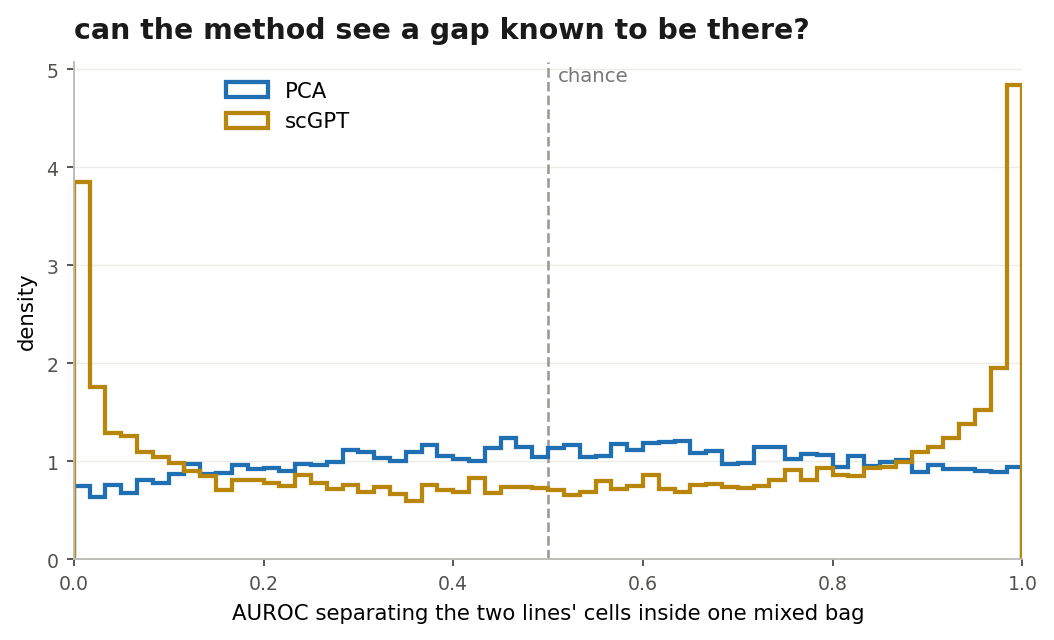
\includegraphics[width=0.78\textwidth]{q2_instrument.png}
\caption{\textbf{Positive control of the heterogeneity criterion.} Distribution of the within-bag area
under the receiver operating characteristic curve (AUROC) with which the MIL model separates the cells of
two mixed cell lines whose response is known to differ, computed as the Mann--Whitney statistic divided
by $n_A n_B$ \cite{mannwhitney1947,hanley1982}; one value per (compound, line pair, seed), $17{,}427$ per
representation, shown as a density histogram for PCA (blue) and scGPT (gold). The dashed line marks
chance (0.5); a value near 1 or 0 means the two populations are ranked apart. Medians: \QAurocPca{}
(PCA), \QAurocScgpt{} (scGPT).
% Read from \code{mil/stage7\_positive\_control.csv}.
}
\label{fig:q2instrument}
\end{figure}
